\section{Comparing translation tables}
\label{sec:translation-tables}

%\begin{figure} [htbp]
%\centering
%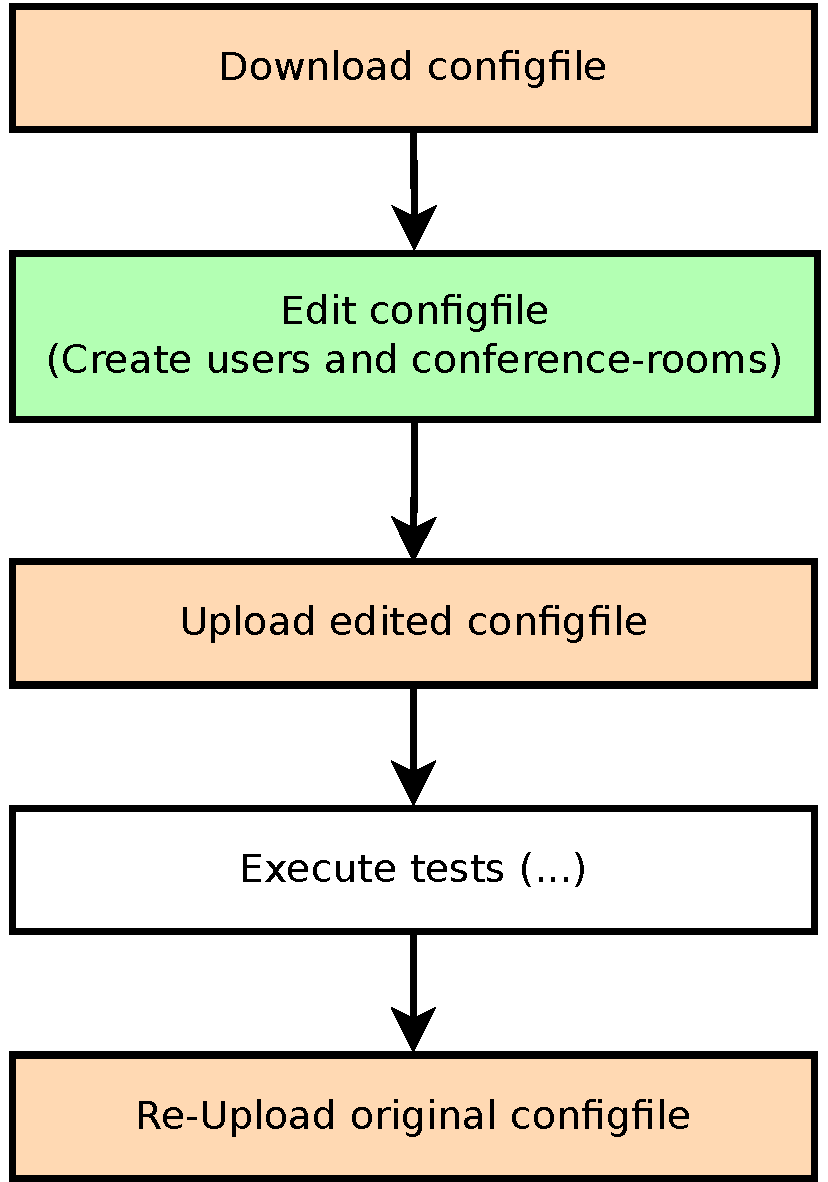
\includegraphics [width=7cm] {configuration-1}
%\caption{Process of editing the Askozia-configuration file}
%\end{figure}

%\begin{tabular}{|p{2cm}|p{12cm}|} \hline
%	\textsc{Test type} & \textsc{Required users} \\ \hline \hline
%	two-way & \texttt{= 2 * 2way-calls} (User A and B for each call) \\
%	conf room & \texttt{= conf-calls-room * conf-rooms-room} \newline (``conf-calls'' users per ``conf-rooms'' conference rooms) \\
%	conf call & \texttt{= conf-calls-call * conf-rooms-call} \newline (``conf-calls'' users per ``conf-rooms'' conference rooms) \\
%	\hline
%\end{tabular}

%\begin{lstlisting}[breaklines=true,label=code:config-user-template,caption={User template} ]
%\end{lstlisting}

This chapter is about a feature that allows the user to show the so called translation table as a bar chart.
A translation table is a list containing the needed conversion times from one codec to another.
The user is able to have a look at the table manually by executing \texttt{core show translation} in the Askozia AMI.
In the following example, the sourcecode is listed in the left column and the destination code in the first row:

\begin {table} [htpb]
\centering
\begin{tabular}{|c|c|c|c|c|} \hline
	 & \textsc{gsm} & \textsc{u-law} & \textsc{a-law} & \textsc{G.722} \\ \hline \hline
	\textsc{gsm} & 0 & 4 & 4 & 9 \\
	\textsc{ulaw} & 10 & 0 & 1 & 6 \\
	\textsc{alaw} & 10 & 1 & 0 & 6 \\
	\textsc{g722} & 19 & 10 & 10 & 0 \\
	\hline
\end{tabular}
\end{table}

\begin{figure} [htbp]
\centering
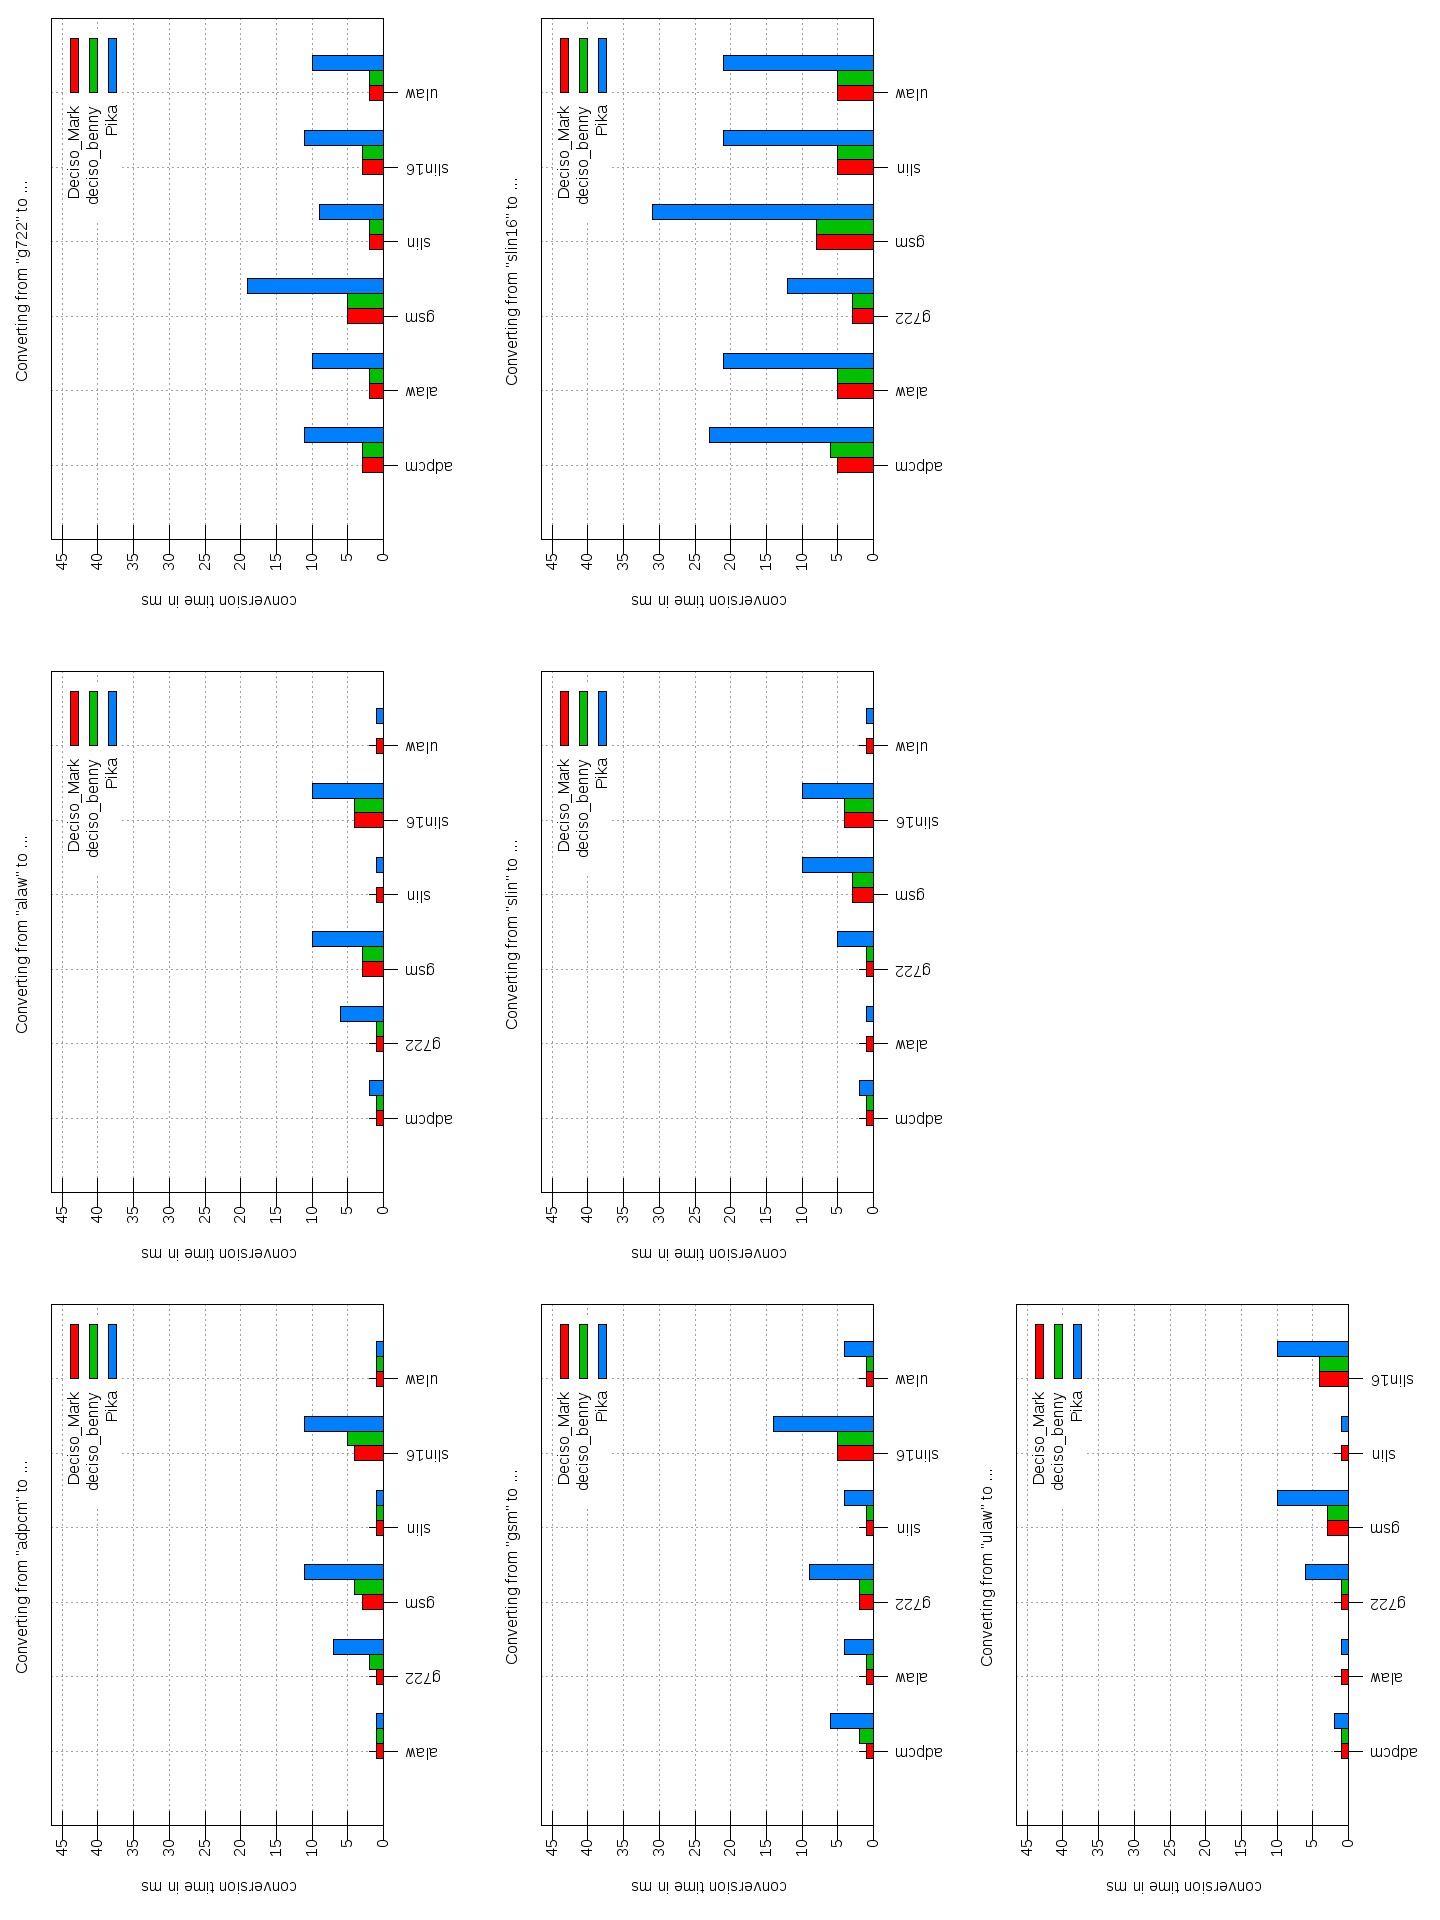
\includegraphics [width=16cm] {translation-tables-1}
\caption{Bar charts of a translation table}
\end{figure}

%%%%%%%%%%%%%%%%%%%%%%%%%%%%%%%%%%%%%
\subsection{Choosing codecs to draw}%
%%%%%%%%%%%%%%%%%%%%%%%%%%%%%%%%%%%%%

The script is able to avoid printing all codecs.
The user can specify a list of the preffered codecs by using the \texttt{-{}-draw-codec} parameter.
It is described in detail in section \ref{sec:introduction}.
This list is used for both source and destination codecs.

%%%%%%%%%%%%%%%%%%%%%%%%%%%%%%%%%%%%%%%%%%
\subsection{Comparing translation tables}%
%%%%%%%%%%%%%%%%%%%%%%%%%%%%%%%%%%%%%%%%%%

It is possible to include other downloaded translation tables in the bar chart for comparing different PBX installations with each other.
For this feature, have a look at the parameter \texttt{-{}-compare-PBX-with} described in section \ref{sec:introduction}.
If some PBX installations can translate different codes, the script draws the codecs provided by the original (tested) PBX installation only.
This list can be edited by the parameter \texttt{-{}-draw-codec}.
